\documentclass[12pt letter]{report}
\input{./template/preamble}
\input{./template/macros}
\input{./template/letterfonts}

\title{\Huge{Transport Layer}}
\author{\huge{Madiba Hudson-Quansah}}
\date{}
\usepackage{parskip}
\usepackage{circuitikz}
\usepackage{listings}
\usepackage{tabularx}

\usetikzlibrary{arrows, positioning, shapes.gates.logic.US,
circuits.logic.US, shapes.misc, automata}

\tikzset{
  ->, % makes the edges directed
  % >=stealth’, % makes the arrow heads bold
  node distance=3cm, % specifies the minimum distance between two
  % nodes. Change if necessary.
  every state/.style={thick, fill=gray!10}, % sets the properties for
  % each ’state’ node
  initial text=$ $, % sets the text that appears on the start arrow
}

\setcounter{tocdepth}{4}
\setcounter{secnumdepth}{4}

\begin{document}
\maketitle
\newpage
\pdfbookmark[section]{\contentsname}{too}
\tableofcontents
\pagebreak

\chapter{Transport Layer Services}

\dfn{Logical Communication}{
  From the application's perspective on two different hosts, the transport layer
  provides an interface that enables communication between the two
  application processes, as if they were directly connected on the same host.
}

A transport layer protocol provides logical communication between
application processes running on different hosts. Transport later
protocols are implemented in the end system on the network edge, not
in routers in the network core. The transport layer converts the
application layer messages it receives from a sending application
process into transport layer packets, i.e. segments, by breaking down
application messages into smaller chunks and adding a transport
header to each chunk.

\section{Transport vs Network Layer}

Whereas a transport layer protocol provides logical communication
between processes running on different hosts, a network layer
protocol provides logical communication between hosts, i.e. the two
hosts can interact as if the were on the same physical network.

\chapter{Multiplexing and Demultiplexing}

Transport layer multiplexing and demultiplexing extend the host to
host delivery service provided by the network layer to a process to
process delivery service for applications running on the hosts.

Because message delivery is not done directly between application
processes but through sockets, there can be multiple sockets in the
receiving host that are receiving messages from the network layer.
The transport layer must have a way to direct each incoming message
to the correct socket, and this is done through multiplexing and demultiplexing.

\dfn{Demultiplexing}{
  The process of delivering the data in a transport layer segment to
  the correct socket.
}

\dfn{Multiplexing}{
  The process of gathering data chunks at the source host from
  different sockets, encapsulating each data chunk with header
  information, i.e. creating segments, and passing the segments to
  the network layer.
}

Multiplexing requires:
\begin{enumerate}
  \item Sockets have unique identifiers, i.e. port numbers.
  \item Each segment have special fields that indicate the socket to
    which the segment was sent from, i.e. source port number, and the
    socket to which the segment is sent to, i.e. destination port number.
\end{enumerate}

\section{Connectionless Multiplexing and Demultiplexing}

When a UDP socket is created the transport layer assigns a port
number to the socket, in the range 1024 to 65535.  When a host A with
a UDP port 1025 wants to send a data chunk to a host B with a UDP
port 2048, the following happens:
\begin{enumerate}
  \item The transport layer in host A create a transport layer
    segment including the data chunk, the source port number 1025,
    the destination port number 2048, and other header information.
    I.e. Multiplexing.
  \item The transport layer passes the segment to the network layer,
    which encapsulates the segment in an IP datagram and makes a
    best-effort attempt to deliver the segment to the host B.
  \item If the segment arrives at host B, the transport layer at host
    B examines the destination port number, in the segment, i.e.
    2048, and delivers the segment to the socket with port number
    2048. I.e. Demultiplexing.
\end{enumerate}

The UDP socket is full identified by a two-tuple made up of the
destination IP address and destination port number, as a consequence
if two IP segments have different source IP addresses and/or source
port numbers, but the same destination IP address and destination
port number, the segments will be delivered to the same socket.

\section{Connection-Oriented Multiplexing and Demultiplexing}

A TCP socket is identified b a four tuple, made up of:
\begin{itemize}
  \item Source IP address
  \item Source Port number
  \item Destination IP address
  \item Destination Port number
\end{itemize}
When a TCP segment arrives from the network to a host B, the host B
examines all for values to demultiplex the segment to the correct
socket. This means that if two arriving TCP segments have different
source IP addresses or source port numbers, than the ones used to
initiate the TCP connection, but the same destination IP address and
destination port number, the segments will not be delivered to the
same socket, with an exception of the TCP segment used to initiate
the TCP connection, which will be delivered to the socket that is
waiting for connection requests. Given a TCP server application
running on host A with a TCP socket with a port number 1025, and a
TCP client application running on host B with a TCP socket with a
port number 2048, when the client application initiates a TCP
connection to the server application, the following happens:
\begin{enumerate}
  \item The host A has a "welcoming socket" with port number 1025
    that waits for connection establishment requests from TCP clients.
  \item The host B create s socket and sends connection establishment
    request to host A, with source port number 2048 and destination
    port number 1025,  establishing the source IP address and
    destination IP address in the TCP segment to the IP addresses of
    host B and host A respectively,
  \item  When the host A receives the incoming connection request
    segment with destination port 1025t locates the welcoming socket
    ad creates a new socket, used to handle the connection with host
    B, with the same port number 1025.
  \item The newly created connection socket in host A is identified b
    the four tuple, and all subsequently arriving TCP segments with
    the same four tuple, will be demultiplexed to the same socket.
\end{enumerate}

\chapter{Connectionless Transport: User Datagram Protocol (UDP)}

UDP is very lightweight as it does the bare minimum a transport
protocol can do, which is providing multiplexing and demultiplexing
and light error checking. UDP encapsulates messages from the
application process into segments, attaching source and destination
port numbers for multiplexing/demultiplexing, and passes it along to
the network layer, where it encapsulates the transport layer segment
into an IP datagram and then makes a best-effort attempt to deliver
the segment to the receiving host. There is no handshaking between
UDP servers and clients so UDP is said to be \textit{connectionless}.
UDP is preferred over TCP in certain situation for the following reasons:
\begin{description}
  \item[Finer application level control over what data is sent nd when]  -
    As soon as an application process basses data to UDP, it is
    encapsulated into a UDP segment and
    immediately passed to the network layer, this differs from all
    the congestion and flow control mechanisms in TCP that throttles
    the transport layer TCP sender when one or more links between the
    source and destination hosts are congested or to regulate the
    rate at which the sender is sending data to the receiver, which
    can cause delays in the delivery of data to the receiving
    application process.
  \item[No connection establishment] - TCP requires a three-way
    handshake before data is transmitted, which can cause delays in
    the delivery of data to the receiving application process,
    whereas UDP does not require a connection establishment phase
    before data is transmitted. This makes it faster than TCP for
    applications that send small amounts of data
  \item[No conneciton state] - TCP maintains connection state in the
    end systems, which includes receive and send buffers,
    congestion=control parameters, and sequence and acknowledgement
    number parameters. UDP however does not maintain connection state
    and does not track any of these parameters, allowing it to
    support more active clients than TCP, which is useful for
    applications that have a large number of clients, such as DNS servers.
  \item[Small packet header overhead] - The TCP segment has 20 bytes
    of header overhead in every segment while UDP only has 8 bytes of overhead.
\end{description}

UDP has no congestion control, which is needed to prevent the network
from entering a congested state which could lead to packet loss and
delays. This means one must be careful when using UDP in a situation
like media streaming where a large amount of data is being sent, as
this could lead to congestion in the network and consequently packet
loss and delays. However, UDP is still preferred over TCP for media
streaming because it is more important to have timely delivery of
data than to have reliable delivery of data, which is what TCP provides.

UDP does not guarantee reliable data transfer, however it is possible
for an application to have reliable data transfer of UDP, by
implementing reliability in the application itself, through
techniques like acknowledgement and retransmission.

\section{UDP Segment Structure}
The width of a UDP segment is 32 bits and the structure is as follows:
\begin{description}
  \item[Source Port Number]  - 16 bits, identifies the sending socket.
  \item[Destination Port Number] - 16 bits, identifies the receiving socket.
  \item[Length] - 16 bits, specifies the length of the UDP segment in bytes,
    including the header and data.
  \item[Checksum] - 16 bits, used for error detection of the UDP segment.
  \item [Data] - Variable length, contains the data from the
    application process.
\end{description}

\section{UDP Checksum}

The UDP checksum is used for error detection, by determining whether
bits within the UDP segment have been altered as it is moved from
source to destination. This is done by the sender computing the
ones-complement of he sum of all the 16-bit words in the UDP segment,
with any overflow being wrapped around, i.e. added to the least
significant bit of the sum. The result is put in the checksum field
of the UDP segment.
\ex{}{
  Given the following 16 bit words:
  \begin{align*}
    0110 \,0110 \,0110 \,0000 \\
    0101 \,0101 \,0101 \,0101 \\
    1000 \,1111 \,0000 \,1100
  \end{align*}
  The sum of the word two words is:
  \begin{align*}
    0110 \,0110 \,0110 \,0000 \\
    0101 \,0101 \,0101 \,0101 \\
    \\
    1011\,1011\,1011\,0101
  \end{align*}
  And adding the third gives us:
  \begin{align*}
    1011\,1011\,1011\,0101\\
    1000 \,1111 \,0000 \,1100
    \\
    0100\,1010\,1100\,0010
  \end{align*}
  Notice there was an overflow which has been wrapped around.
  We then ones-complement the result giving us $1011010100111101$,
  which becomes the checksum.
}

At the receiving end all four four 16-bit words are added including
the checksum, if no errors occurred then the sum at the receiver
should be all ones, i.e. $1111 \,1111 \,1111 \,1111$. If the sum is
not all ones then an error has occurred and the segment is discarded.

\dfn{End-to-End Principle}{
  The principle that states that since certain functionality must be
  implemented on an end-to-end basis, function placed at the lower
  levels may be redundant or of little value when compared to the
  cost of providing them at the higher level.
}

UDP most provide error detection at the transport layer on an
end-to-end bases if the end-end data transfer service is to provide
error detection, this is an example of the \textbf{end-to-end principle}.

\chapter{Principles of Reliable Data Transfer}

It is the  responsibility of a reliable data transfer protocol to
implement this service by using the unreliable data transfer service
provided by the network layer. The network layer's IP protocol is an
unreliable end-to-end data transfer service, which means that the
network layer may lose packets, may corrupt packets, and may deliver
packets out of order. We make the assumption that packets are
delivered in the order that they are sent, with some packets possibly
being lost along the way.

We also only consider the case unidirectional data transfer, where
data is only sent from a sender to a receiver, nonetheless packets
will still be transmitted in both directions, as the receiver will
send acknowledgement packets back to the sender to acknowledge the
receipt of data.

\section{Reliable Data Transfer Protocol Techniques}

\subsection{Reliable Data Transfer over a Perfectly Reliable Channel (rdt1.0)}

We first consider the case where the underlying channel is completely
reliable, putting this into context, the network layer's IP protocol
is considered to be completely reliable which is not the case.

Both the sender and receiver go through various states based on the
events that occur and the packets passed between them.

\begin{figure}[H]
  \centering
  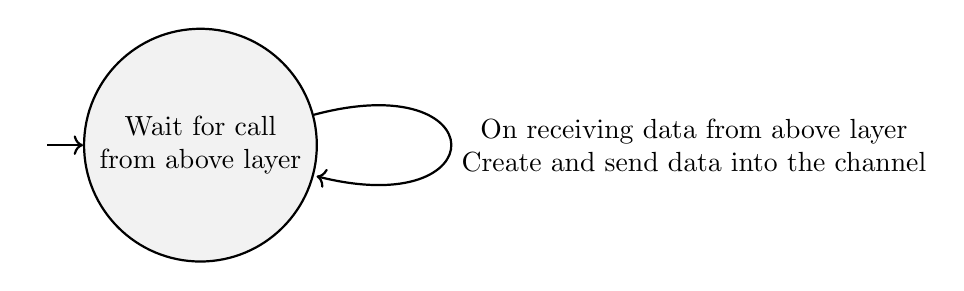
\begin{tikzpicture}[node distance={3cm},thick,main/.style = {draw, circle}]

    \node[state, initial, align=center] (wait)  {Wait for call\\from
    above layer};

    \draw
    (wait) edge[loop right] node[align=center] {On receiving data
      from above layer\\Create and send data into the channel
    } (wait)
    ;
  \end{tikzpicture}
  \caption{rdt1.0 sender}
\end{figure}

\begin{figure}[H]
  \centering
  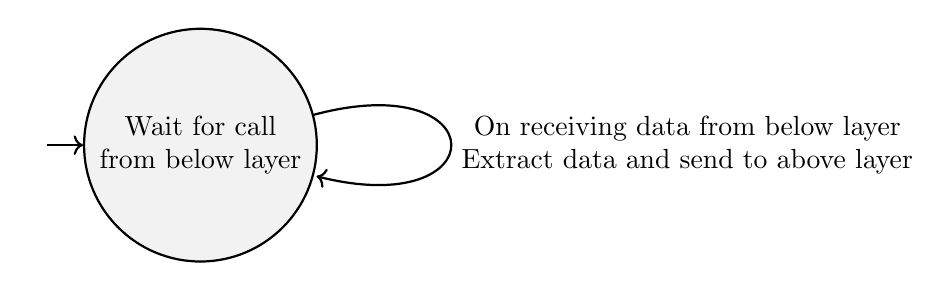
\begin{tikzpicture}[node distance={3cm},thick,main/.style = {draw, circle}]

    \node[state, initial, align=center] (wait)  {Wait for call\\from
    below layer};

    \draw
    (wait) edge[loop right] node[align=center] {On receiving data
      from below layer\\Extract data and send to above layer
    } (wait)
    ;
  \end{tikzpicture}
  \caption{rdt1.0 receiver}
\end{figure}

The sender accepts data from the upper layer, in this case the
application layer, and encapsulates the data and sends the packet
into the reliable channel.

The receiver waits for a packet to arrive from the underlying
channel, extracts the data from the packet and passes the data up to
the upper layer, in this case the application layer.

In this we use the terms data and packet interchangeably because
there is no difference between the two, as there is no header
information added to the data to create a packet, as the channel is
perfectly reliable and there is no need for any header.

In a perfectly reliable channel there is no need for the receiver to
acknowledge receipt of data because the sender can be assured that
the data will be delivered to the receiver without any errors, and
there is no need for the sender to retransmit data because the sender
can be assured that the data will not be lost in the channel.

\subsection{Reliable Data Transfer over a Channel with Bit Errors (rdt2.0)}

In this case the bits sent though the underlying channel by become
corrupted, typically occurring in the physical components of a
network as a packet is transmitted, propagates or is buffered. We
still assume packets are received in the order they are sent.

\dfn{Positive Acknowledgement}{
  An acknowledgement sent by the receiver to the sender to indicate
  that a packet was received without any errors.
}

\dfn{Negative Acknowledgement}{
  An acknowledgement sent by the receiver to the sender to indicate
  that a packet was received with errors.
}

In this case where errors may occur in transmission, the receiver
must be able to acknowledge the receipt of corrupted or valid data,
with \textbf{negative} and \textbf{positive} acknowledgements
respectively, and the sender must be able to retransmit data when it
receives a negative acknowledgement. Reliable data transfer protocols
based on retransmission are known as \textbf{Automatic Repeat reQuest
(ARQ)} protocols. Generally ARQ protocols must have the following capabilities:
\begin{description}
  \item[Error Detection]  - A mechanism on the receiver side to
    detect when bit errors have occurred, for example, checksums.
  \item[Receiver Feedback] - The receiver must be able to provide
    explicit feedback to the sender about whether a packet was
    received with or without errors, for example, through positive
    (ACK) and negative (NAK) acknowledgements.
  \item[Retransmission] - A packet that is received in error at the
    receiver will be retransmitted by the sender.
\end{description}

\begin{figure}[H]
  \centering
  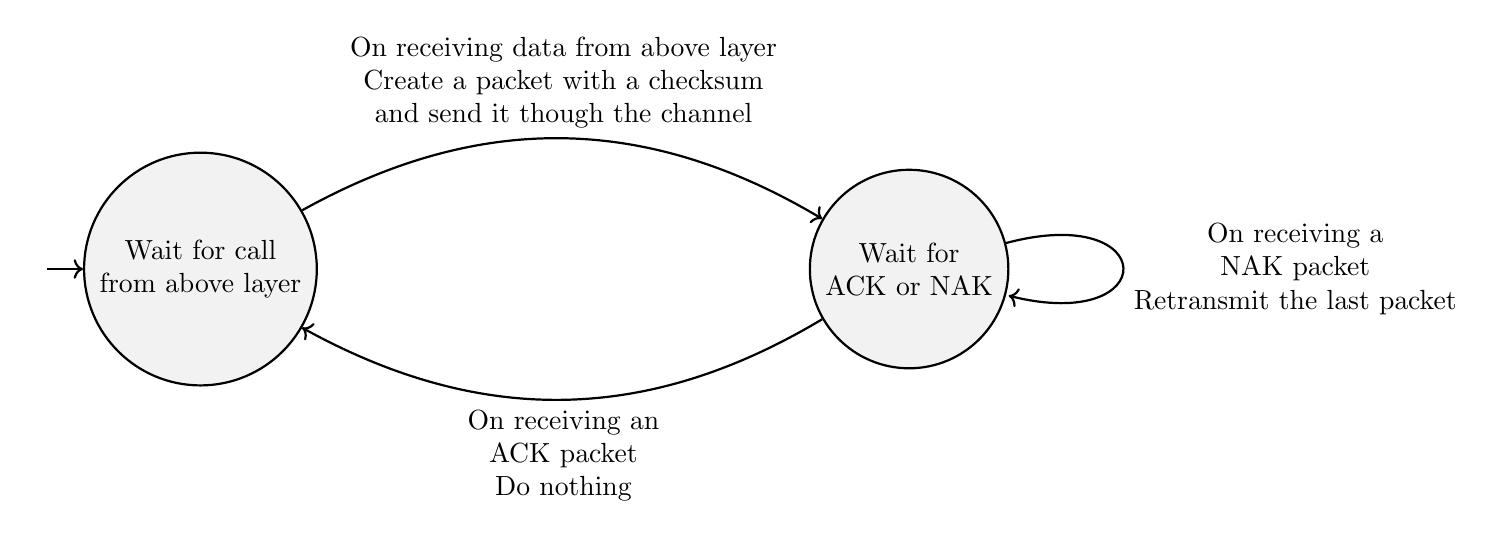
\begin{tikzpicture}[node distance={9cm},thick,main/.style = {draw, circle}]
    \node[state, initial, align=center] (layer) {Wait for call\\from
    above layer};
    \node[state, right of=layer, align=center] (nack) {Wait for\\ACK or NAK};

    \draw
    (layer) edge[bend left, above] node[align=center] {On receiving
      data from above
      layer\\Create a packet with a checksum\\and send it though the
    channel} (nack)

    (nack) edge[loop right] node[align=center] {On receiving a\\NAK
    packet\\Retransmit the last packet } (nack)

    (nack) edge[bend left, below] node[align=center] {On receiving an\\ACK
    packet\\Do nothing} (layer)

    ;
  \end{tikzpicture}
  \caption{rdt2.0 sender}
\end{figure}

\begin{figure}[H]
  \centering
  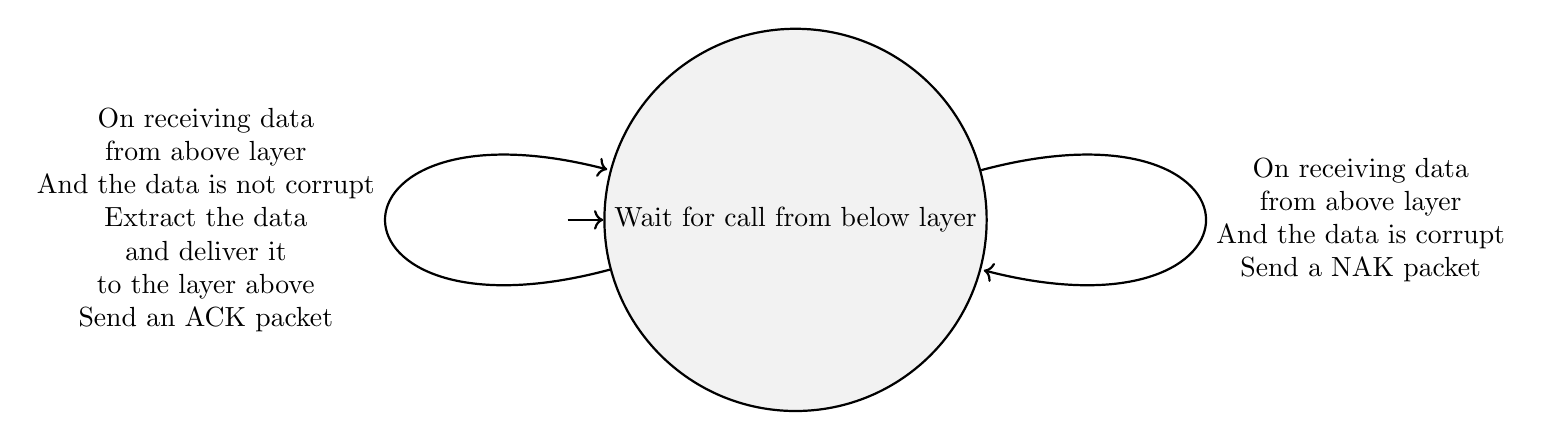
\begin{tikzpicture}[node distance={3cm},thick,main/.style = {draw, circle}]
    \node[state, initial] (wait) {Wait for call from below layer};

    \draw
    (wait) edge[loop right] node[align=center] {On receiving data\\
    from above layer\\And the data is corrupt\\Send a NAK packet} (wait)
    (wait) edge[loop left]  node[align=center] {On receiving
      data\\from above layer\\And the data is not corrupt\\Extract the
    data\\and deliver it\\to the layer above\\Send an ACK packet} (wait)

    ;
  \end{tikzpicture}
  \caption{rdt2.0 receiver}
\end{figure}

The sender side of rdt2.0 has two states, waiting for data from the
above layer, and waiting for ACKs/NAKs.

When data is received from
the above layer the sender creates a packet along with a packet
checksum and sends the packet through the channel.

When the sender is waiting for an ACK/NAK from the receiver, if an
ACK is received the sender knows the most recently transmitted packet
has been received correctly  and can return to the waiting for data
state. If a NAK is received the protocol retransmits the last packet
and waits for an ACK/NAK to be transmitted in response to the
retransmitted data. When the sender is in the waiting for
acknowledgement state it cannot receive data from the above layer,
and cannot send a new packet until it is sure that the receiver has
correctly the current packet. This feature marks rdt2.0 as a
\textbf{stop-and-wait} protocol

The receiver side only has a single state, the waiting for data from
below layer state. On receiving  packet the receiver transmits either
an ACK or NAK depending on whether or not the packet is corrupted.

\subsubsection{Corrupt Acknowledgements}

rdt2.0 has a major disadvantage however, the fact that it does not
count for the possibility that that the ACK/NAK sent by the receiver
is corrupted. Adding checksums to the acknowledgement packets can
help, but the sender has no way of knowing whether or not the
receiver has correctly received the last piece of transmitted data.
There are three possibilities for handling corrupted acknowledgements

\begin{description}
  \item[The sender requests another acknowledgement after sometime]
    - If the sender waits a while and does not receive an
    acknowledgement the sender could send a message requesting an
    acknowledgement introducing a new type of sender-to-receiver
    packet. But this new type of packet could also become corrupted,
    and the receiver could have no way of identifying the type of the
    received corrupted packet, ad infinitum.
  \item[Add enough checksum bits to allow the sender to both detect
    and recover from bit errors]-
    This solves the immediate problem for a channel that can corrupt
    messages but not lose them.
  \item[The sender retransmits the current data when it receives a
    corrupted acknowledgement] - This approach however introduces
    duplicate packets into the channel, the receiver doesn't know
    whether the ACK/NAK it last send was received correctly at the
    sender, thus it cannot know a priori whether an arriving packet
    contains new data or is a retransmission.
\end{description}

A solution to the duplicate packet problem is to attach a
\textbf{sequence number} to the data packet. The receiver then only
needs to check the sequence number to determine whether or not the
received packet is a retransmission. This is where rdt2.1 comes into play.

\subsubsection{rdt2.1}

In rdt2.1 we use a 1-bit sequence number to distinguish between new
data and retransmissions, the sender alternates between sequence
numbers 0 and 1 for each new data packet it sends. The receiver only
accepts packets with the expected sequence number, if a packet with
an unexpected sequence number is received, the receiver sends a NAK
and discards the packet, if a packet with the expected sequence number
is received, the receiver sends an ACK and delivers the data to the
application layer. This leads to a more complex FSM for both the
sender and receiver, as the sender has to keep track of the sequence
number of the last packet it sent, and the receiver has to keep track
of the expected sequence number of the next packet it receives.

\begin{figure}[H]
  \centering
  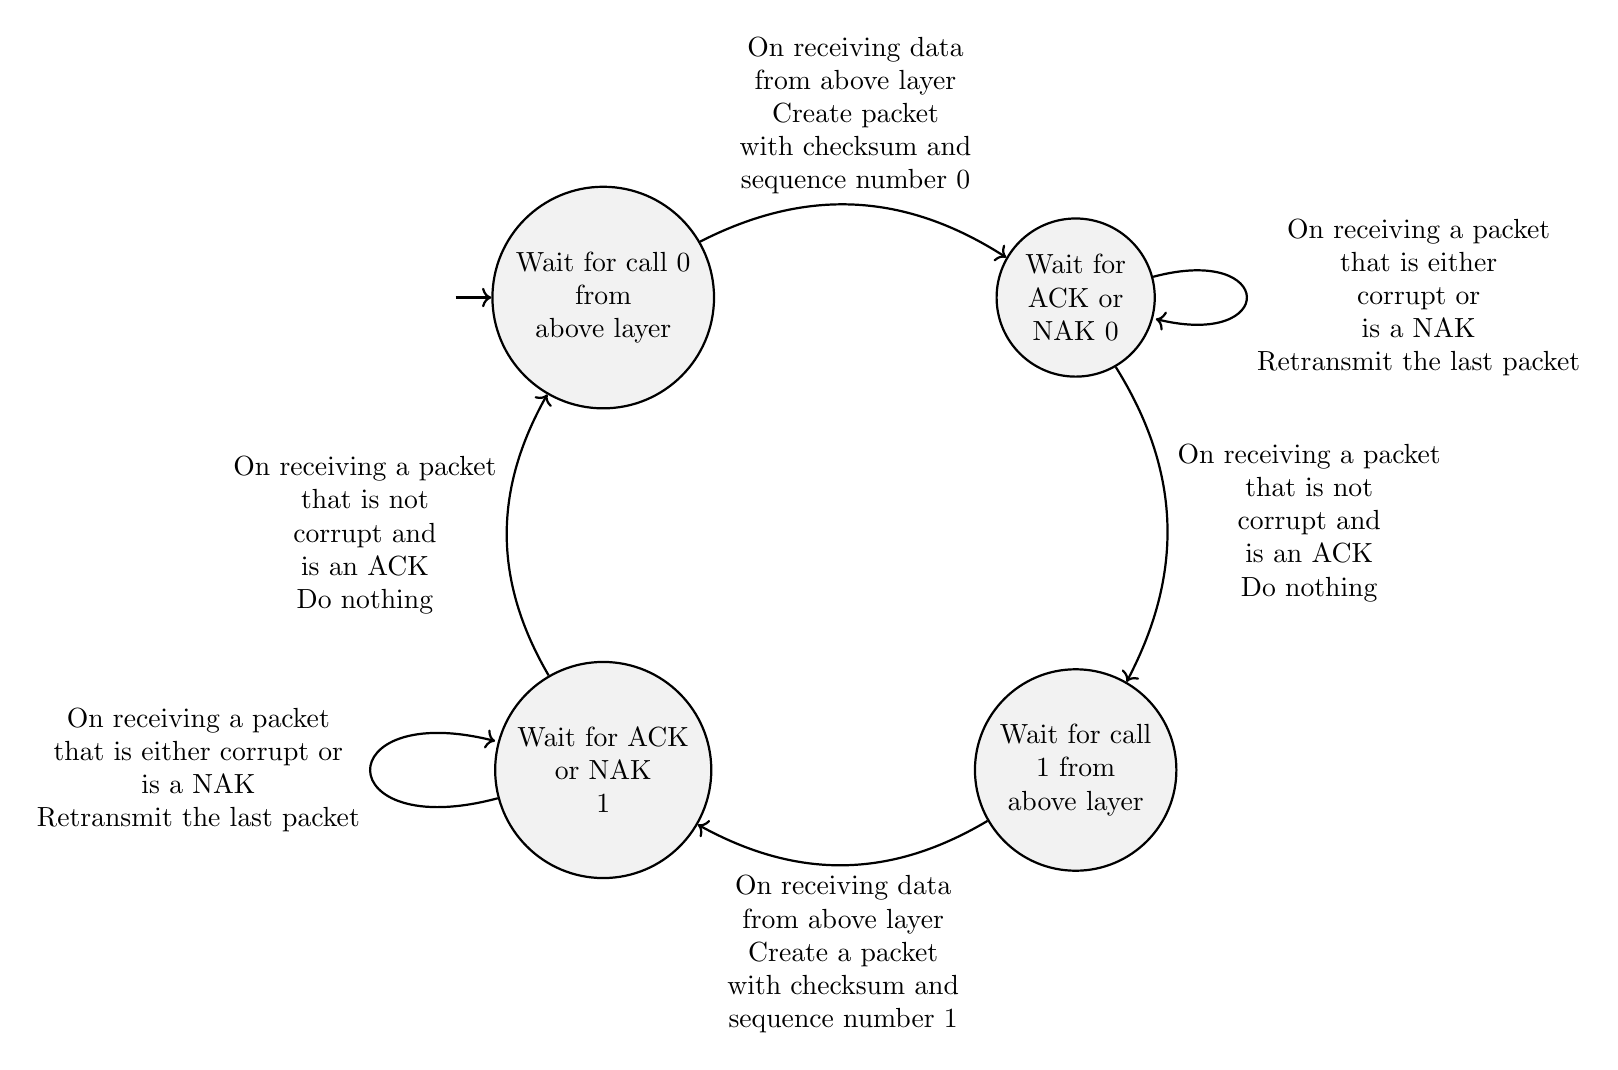
\begin{tikzpicture}[node distance={6cm},thick,main/.style = {draw, circle}]
    \node[state, initial, align=center] (layer_0) {Wait for call 0\\
      from \\
    above layer};
    \node[state, right of=layer_0, align=center] (nack_0) {Wait
    for\\ACK or\\ NAK 0};
    \node[state, below of=nack_0, align=center] (layer_1) {Wait for
      call\\1 from \\
    above layer};
    \node[state, left of=layer_1, align=center] (nack_1) {Wait for
    ACK\\or NAK\\ 1};

    \draw
    (layer_0) edge[bend left, above] node[align=center] {On receiving
      data\\from above layer\\Create packet\\with checksum
    and\\sequence number 0} (nack_0)

    (nack_0) edge[loop right] node[align=center] {On receiving a
      packet\\that is either\\corrupt or\\ is a NAK\\Retransmit the last packet
    } (nack_0)

    (nack_0) edge[bend left, right] node[align=center] {On receiving a
      packet\\that is not\\corrupt and \\is an ACK\\Do nothing
    } (layer_1)

    (layer_1) edge[bend left, below] node[align=center] {On receiving
      data\\from above layer\\Create a packet\\with checksum
      and\\sequence number 1
    } (nack_1)

    (nack_1) edge[loop left] node[align=center] {
      On receiving a packet\\ that is either corrupt or\\is a
      NAK\\Retransmit the last packet
    } (nack_1)

    (nack_1) edge[bend left, left] node[align=center] {
      On receiving a packet\\that is not\\corrupt and\\is an ACK\\Do nothing
    } (layer_0)

    ;
  \end{tikzpicture}
  \caption{rdt2.1 sender}
\end{figure}

\begin{figure}[H]
  \centering
  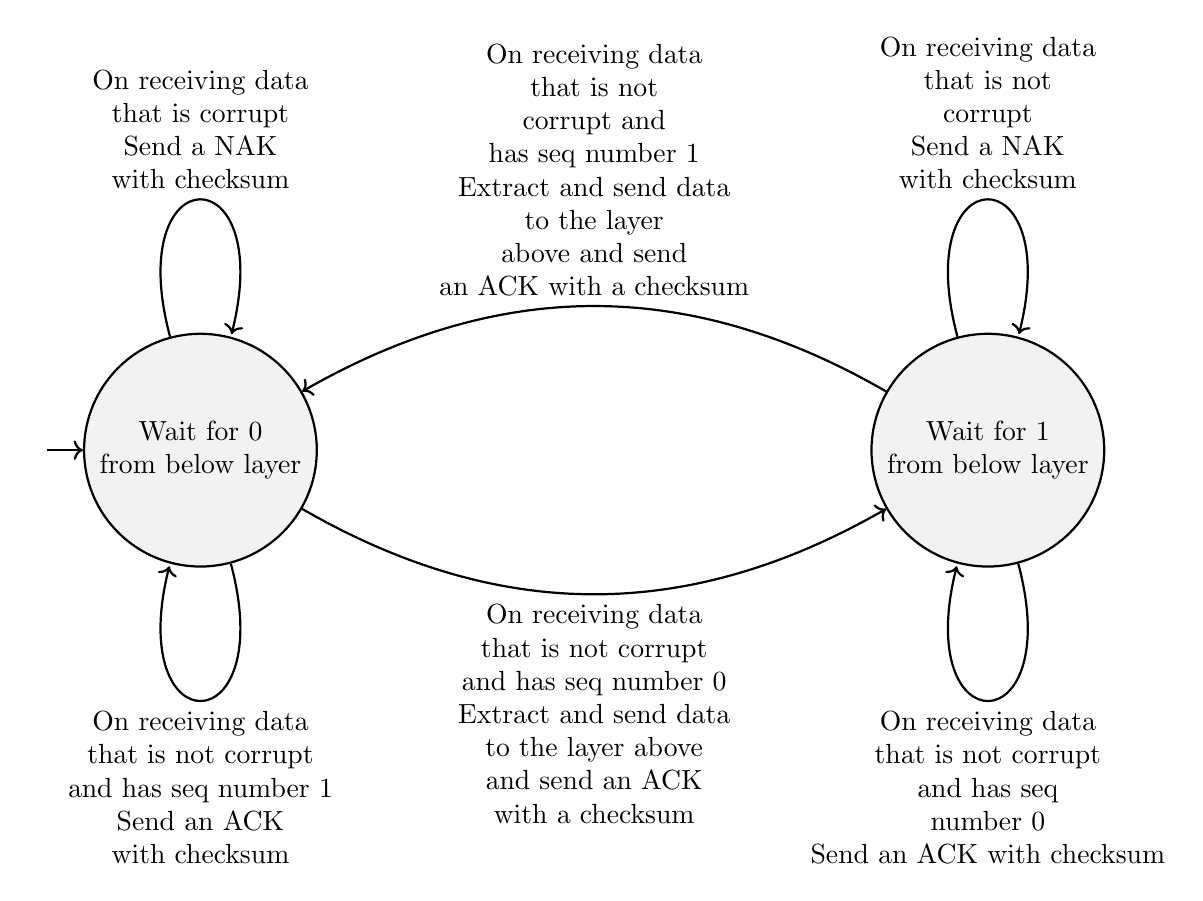
\begin{tikzpicture}[node distance={10cm},thick,main/.style = {draw, circle}]
    \node[state, initial, align=center] (wait_0) {Wait for 0\\from below layer};
    \node[state, right of=wait_0, align=center] (wait_1) {Wait for
    1\\from below layer};

    \draw
    (wait_0) edge[bend right, below] node[align=center] {On receiving
      data\\that is not corrupt\\and has seq number 0\\Extract and send
    data\\to the layer above\\and send an ACK\\ with a checksum} (wait_1)

    (wait_1) edge[loop above] node[align=center] {On receiving
    data\\that is not\\corrupt\\Send a NAK\\ with checksum} (wait_1)

    (wait_1) edge[loop below] node[align=center] {On receiving
      data\\that is not corrupt\\and has seq \\number 0\\Send an ACK with
    checksum} (wait_1)

    (wait_0) edge[loop above] node[align=center] {On receiving
    data\\that is corrupt\\Send a NAK\\with checksum} (wait_0)

    (wait_0) edge[loop below] node[align=center] {On receiving
      data\\that is not corrupt\\and has seq number 1\\Send an
    ACK\\with checksum} (wait_0)

    (wait_1) edge[bend right, above] node[align=center] {On receiving
      data\\that is not\\corrupt and\\has seq number 1\\Extract and
    send data\\to the layer\\above and send\\an ACK with a checksum} (wait_0)

    ;
  \end{tikzpicture}
  \caption{rdt2.1 receiver}
\end{figure}

rdt2.1 uses both positive and negative acknowledgements from the
receiver to sender. When an out-of-order packet is received, the
receiver sends a positive acknowledgement for the packet it has
received. When a corrupted packet is received the receiver sends a
negative acknowledgement.

\subsubsection{rdt2.2}

We can have the same effect as a NAK, if instead of sending a NAK,
we send an ACK for the last correctly received packet. A sender that
receives two ACKs for the same packet, i.e. duplicate ACKs, knows
that receiver did not correctly receive the packet following the packet
that is being ACKed twice. This NAK free reliable data transfer protocol
for a channel with bit errors is rdt2.2.

A difference between rdt2.1 and rdt2.2 is that receiver must include
the sequence number of the packet being acknowledged by an ACK
message, i.e. including the ACK 0 or 1 when making the packet, and
the sender must check the sequence number of the packet being
acknowledged by a received ACK message.

\begin{figure}[H]
  \centering
  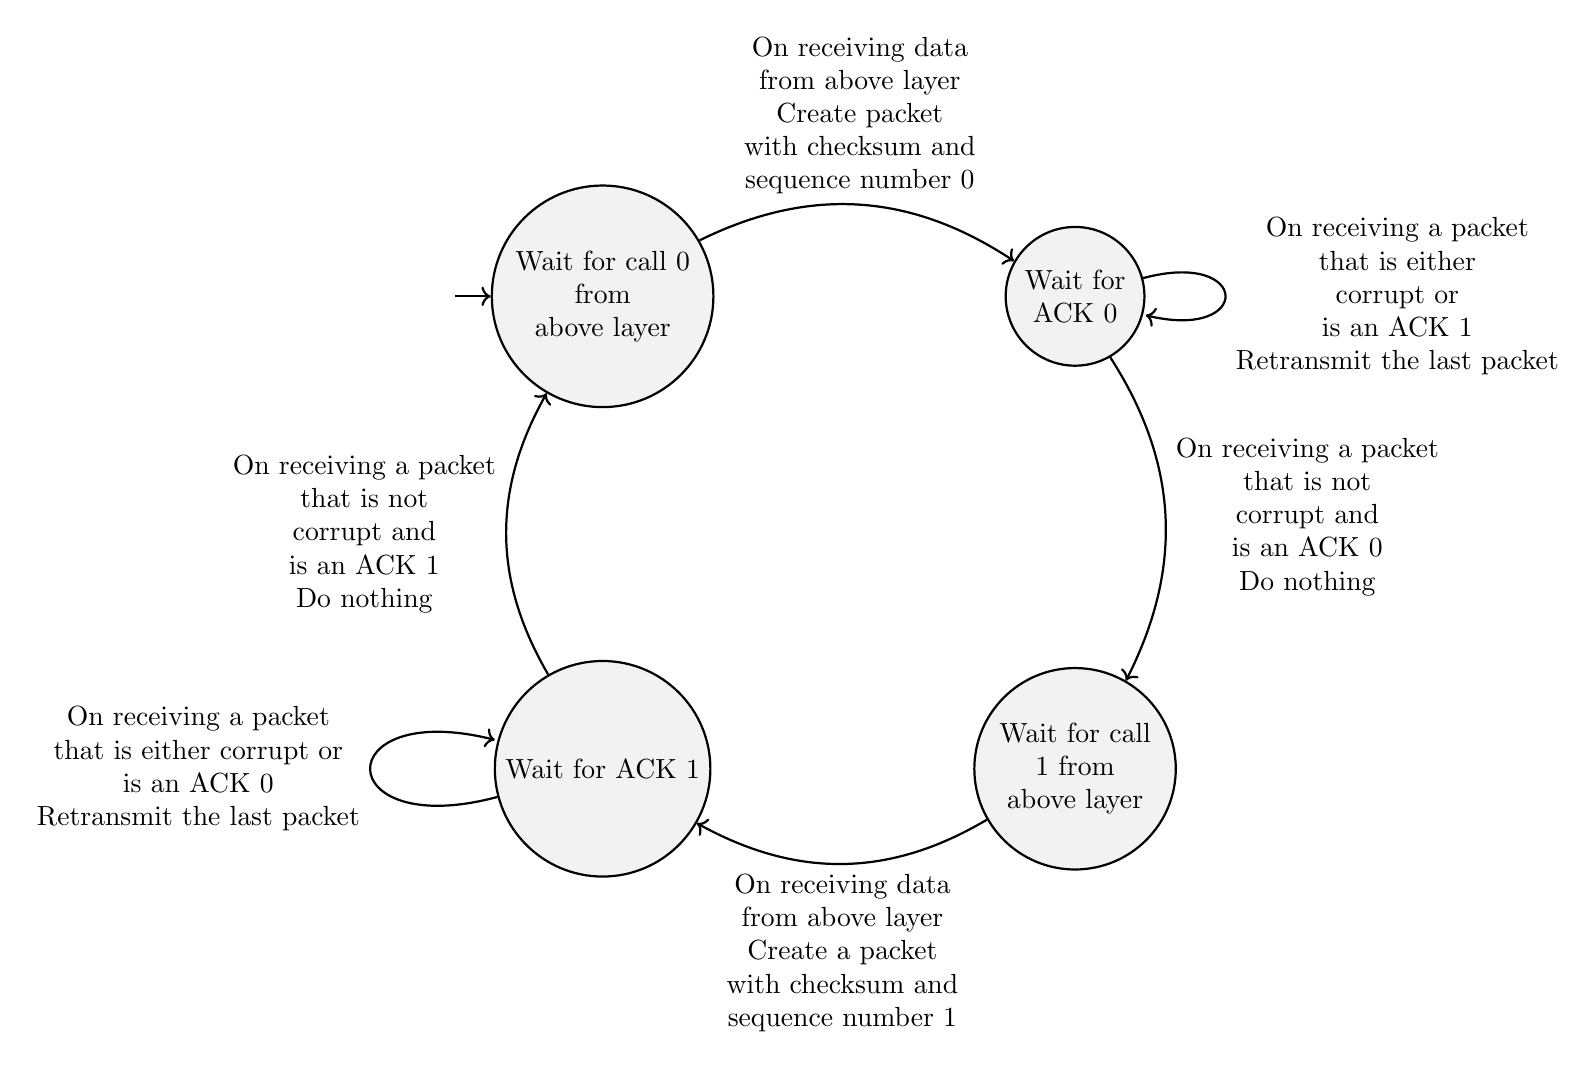
\begin{tikzpicture}[node distance={6cm},thick,main/.style = {draw, circle}]
    \node[state, initial, align=center] (layer_0) {Wait for call 0\\
      from \\
    above layer};
    \node[state, right of=layer_0, align=center] (ack_0) {Wait
    for\\ACK 0};
    \node[state, below of=ack_0, align=center] (layer_1) {Wait for
      call\\1 from \\
    above layer};
    \node[state, left of=layer_1, align=center] (ack_1) {Wait for
    ACK 1};

    \draw
    (layer_0) edge[bend left, above] node[align=center] {On receiving
      data\\from above layer\\Create packet\\with checksum
    and\\sequence number 0} (ack_0)

    (ack_0) edge[loop right] node[align=center] {On receiving a
      packet\\that is either\\corrupt or\\ is an ACK 1\\Retransmit
      the last packet
    } (ack_0)

    (ack_0) edge[bend left, right] node[align=center] {On receiving a
      packet\\that is not\\corrupt and \\is an ACK 0\\Do nothing
    } (layer_1)

    (layer_1) edge[bend left, below] node[align=center] {On receiving
      data\\from above layer\\Create a packet\\with checksum
      and\\sequence number 1
    } (ack_1)

    (ack_1) edge[loop left] node[align=center] {
      On receiving a packet\\ that is either corrupt or\\is an
      ACK 0\\Retransmit the last packet
    } (ack_1)

    (ack_1) edge[bend left, left] node[align=center] {
      On receiving a packet\\that is not\\corrupt and\\is an ACK 1\\Do nothing
    } (layer_0)

    ;
  \end{tikzpicture}
  \caption{rdt2.2 sender}
\end{figure}

\begin{figure}[H]
  \centering
  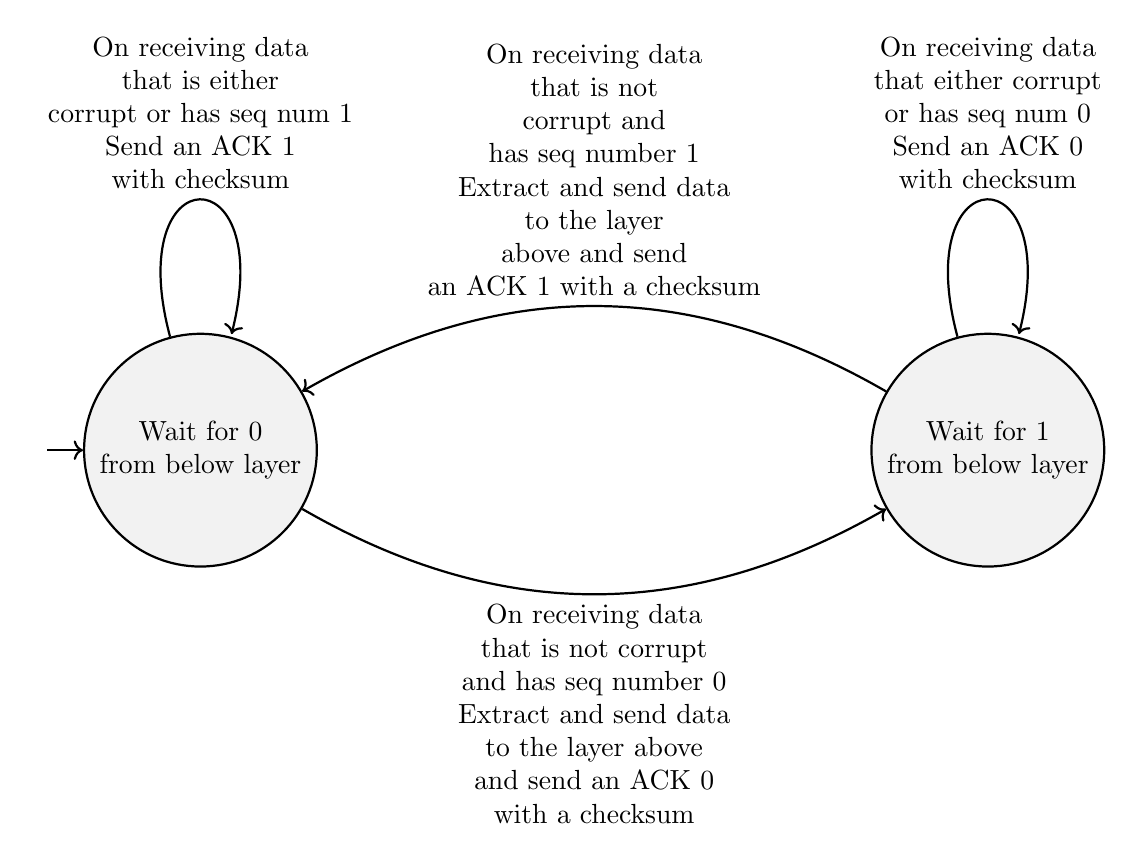
\begin{tikzpicture}[node distance={10cm},thick,main/.style = {draw, circle}]
    \node[state, initial, align=center] (wait_0) {Wait for 0\\from below layer};
    \node[state, right of=wait_0, align=center] (wait_1) {Wait for
    1\\from below layer};

    \draw
    (wait_0) edge[bend right, below] node[align=center] {On receiving
      data\\that is not corrupt\\and has seq number 0\\Extract and send
    data\\to the layer above\\and send an ACK 0\\ with a checksum} (wait_1)

    (wait_1) edge[loop above] node[align=center] {On receiving
      data\\that either corrupt \\
    or has seq num 0\\Send an ACK 0\\with checksum } (wait_1)

    (wait_0) edge[loop above] node[align=center] {On receiving
      data\\that is either\\corrupt or has seq num 1\\Send an ACK
    1\\with checksum} (wait_0)

    (wait_1) edge[bend right, above] node[align=center] {On receiving
      data\\that is not\\corrupt and\\has seq number 1\\Extract and
    send data\\to the layer\\above and send\\an ACK 1 with a checksum} (wait_0)

    ;
  \end{tikzpicture}
  \caption{rdt2.2 receiver}
\end{figure}

\subsection{Reliable Data Transfer over a Lossy Channel with Bit
Errors (rdt3.0)}

Now we disregard the assumption that the underlying channel cannot
lose bits, now the packets can be lost and may be corrupted, this
reflects the common situation for most real life networks.

Two additional concerns must now be addressed by the protocol:
\begin{enumerate}
  \item How to detect packet loss
  \item What to do when packet loss occurs, i.e. Checksums, sequence
    numbers, ACK packets, retransmissions.
\end{enumerate}

We put the burden of detecting and recovering from packet loss on the
sender. In the case a sender sends a packet and waits for an
acknowledgement to send the next packet that never comes, if the
sender is willing to wait long enough so that it is certain that a
packet is lost, it can retransmit the data packet.

The sender must wait at least as long as a round-trip delay between
the sender and receiver, which may include buffering at intermediate
routers, plus whatever amount of time is needed to process a packet
at the receiver. Moreover the protocol should recover from packet
loss as soon as possible, waiting for a worst-case delay could mean a
long wait until error recovery is trigged.

The adopted approach is for the sender to choose a set time value
such that packet loss is likely, although not guaranteed, to have
happened. If an ACK is not received within this time the packet is
retransmitted. This introduces the possibility of duplicate data
packets being received at the receiver, which can be handled by using
sequence numbers as in rdt2.1 and rdt2.2. This therefore requires a
\textbf{countdown timer} that can interrupt the sender after a given
amount of time has expired allowing it to retransmit the packet. The
sender must thus:
\begin{enumerate}
  \item Start a timer each time a packet is sent, after a first-time
    packet or retransmission.
  \item Respond to a timer interrupt by retransmitting the packet
    that caused the timer to start.
  \item Stop the timer when an ACK is received for the packet that caused it.
\end{enumerate}

\begin{figure}[H]
  \centering
  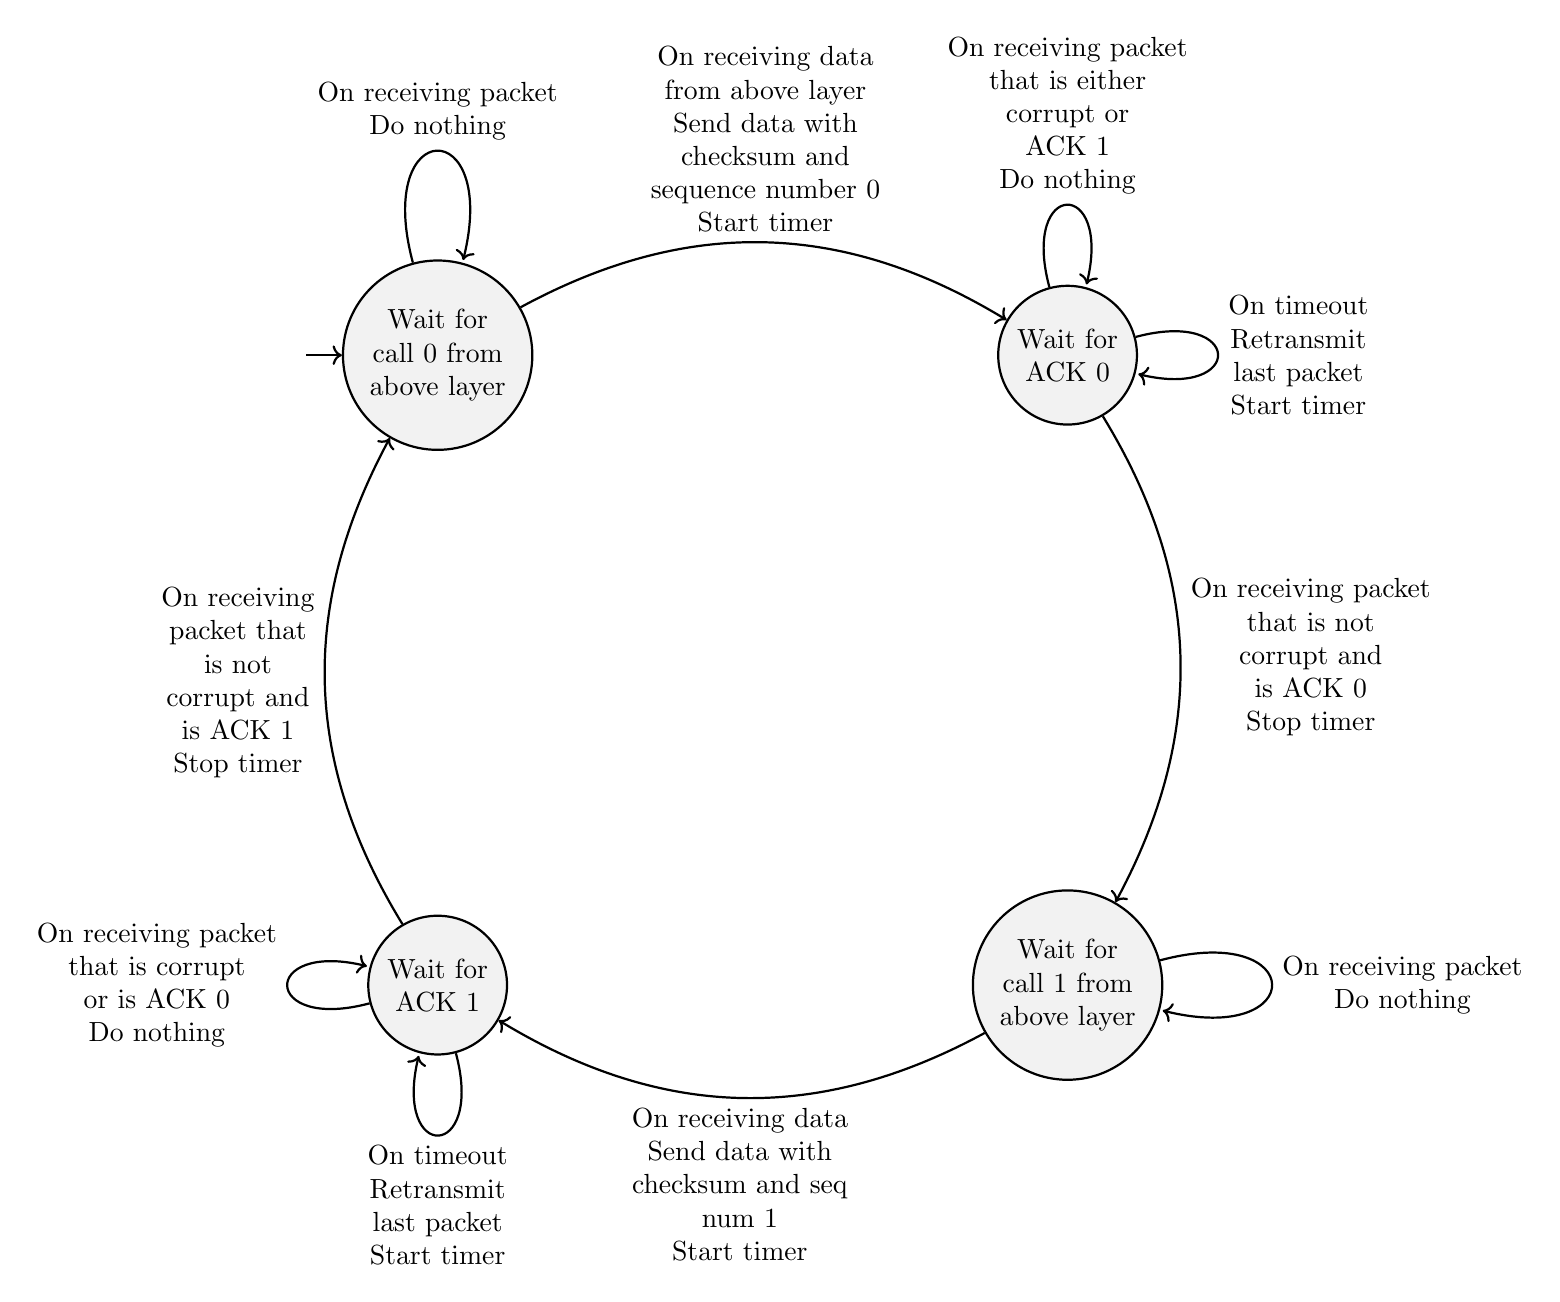
\begin{tikzpicture}[node distance={8cm},thick,main/.style = {draw, circle}]
    \node[state, initial, align=center] (layer_0) {Wait for\\call 0
    from\\above layer};
    \node[state, right of=layer_0, align=center] (ack_0) {Wait for\\ACK 0};
    \node[state, below of=ack_0 , align=center] (layer_1) {Wait
    for\\call 1 from\\above layer};
    \node[state, left of=layer_1, align=center] (ack_1) {Wait for\\ACK 1};

    \draw
    (layer_0) edge[bend left, above] node[align=center] {On receiving
      data\\from above layer\\Send data with\\checksum and \\
    sequence number 0\\Start timer} (ack_0)

    (layer_0) edge[loop above] node[align=center] {On receiving
    packet\\Do nothing} (layer_0)

    (ack_0) edge[loop above] node[align=center] {On receiving
    packet\\that is either\\corrupt or\\ACK 1\\Do nothing} (ack_0)
    (ack_0) edge[loop right] node[align=center] {On
    timeout\\Retransmit\\last packet\\Start timer} (ack_0)

    (ack_0) edge[bend left, right] node[align=center] {On receiving
    packet\\that is not\\corrupt and\\is ACK 0\\Stop timer} (layer_1)

    (layer_1) edge[loop right] node[align=center] {On receiving
    packet\\Do nothing} (layer_1)

    (layer_1) edge[bend left, below] node[align=center] {On receiving
    data\\Send data with\\checksum and seq\\num 1\\Start timer} (ack_1)

    (ack_1) edge[loop below] node[align=center] {On
    timeout\\Retransmit\\last packet\\Start timer} (ack_1)
    (ack_1) edge[loop left] node[align=center] {On receiving
    packet\\that is corrupt\\ or is ACK 0\\Do nothing} (ack_1)

    (ack_1) edge[bend left, left] node[align=center] {On receiving\\packet
    that\\is not\\corrupt and\\is ACK 1\\Stop timer} (layer_0)

    ;
  \end{tikzpicture}
  \caption{rdt3.0 sender}
\end{figure}

\begin{figure}[H]
  \centering
  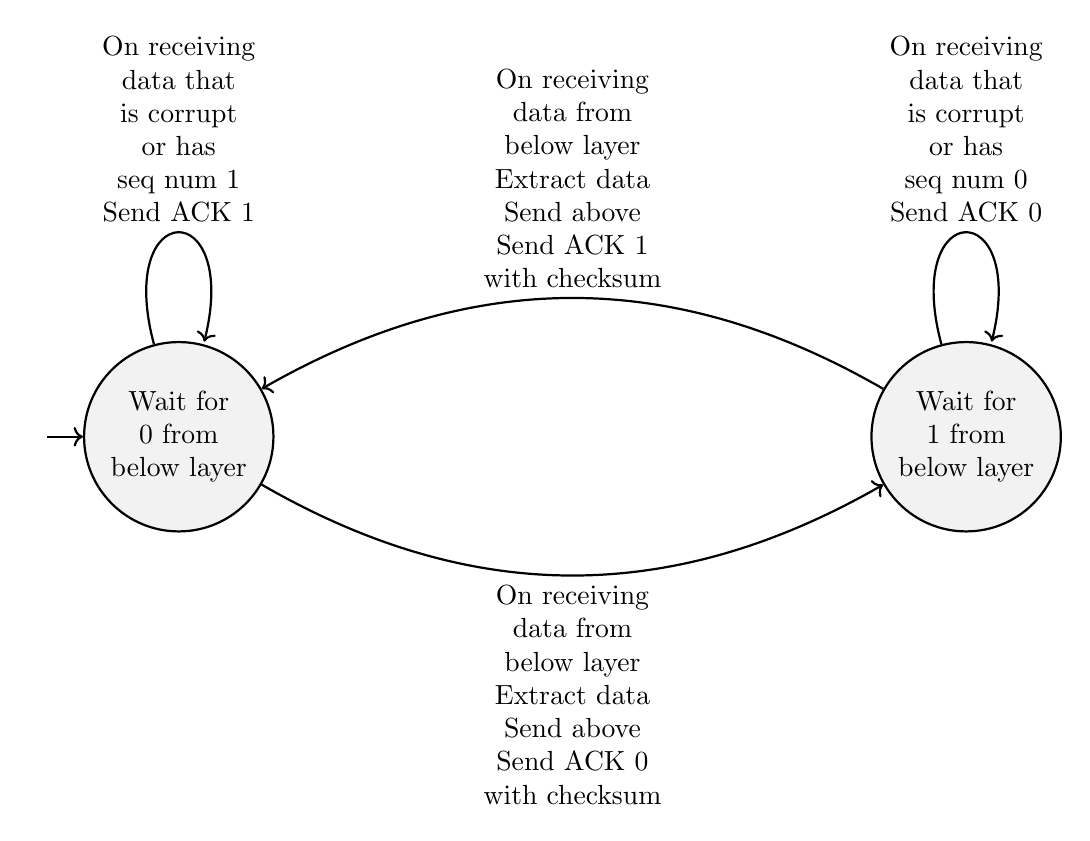
\begin{tikzpicture}[node distance={10cm},thick,main/.style = {draw, circle}]
    \node[state, initial, align=center] (wait_0) {Wait for\\0
    from\\below layer};
    \node[state, right of=wait_0, align=center] (wait_1) {Wait for\\1
    from\\below layer};

    \draw
    (wait_0) edge[bend right, below] node[align=center] {On receiving\\data
      from\\below layer\\Extract data\\Send above\\Send ACK 0\\with
    checksum} (wait_1)

    (wait_0) edge[loop above] node[align=center] {On receiving\\data
    that\\is corrupt\\or has\\seq num 1\\Send ACK 1} (wait_0)

    (wait_1) edge[loop above] node[align=center] {On receiving\\data
    that\\is corrupt\\or has\\seq num 0\\Send ACK 0} (wait_1)

    (wait_1) edge[bend right, above] node[align=center] {On receiving\\data
      from\\below layer\\Extract data\\Send above\\Send ACK 1\\with
    checksum} (wait_0)

    ;
  \end{tikzpicture}
  \caption{rdt3.0 receiver}
\end{figure}

The rdt3.0 reliably transfers data over a channel that can lose and
corrupt packets, handling both issues through the use of checksums,
sequence numbers, acknowledgements, retransmissions and timers.

The sender side of rdt3.0 has four states waiting for either call 0
or 1 from the above layer, and waiting for either ACK 0 or 1 from the
receiver. In its initial state, waiting for call 0, when data is
received the sender makes a packet with sequence number 0 and a
checksum, sends the packet through the channel and starts a timer,
moving on to the next state, waiting for ACK 0.

When the sender in waiting for ACK 0, receives a packet that is
either corrupt or an ACK 1, it does nothing, but when it receives a
packet that is not corrupt and is an ACK 0, it stops the timer and
moves on to the next state, waiting for call 1. The timer timing out
while the sender is still in state waiting for ACK 0, cause the
sender to retransmit the last packet and start the timer again.

When the sender is in state waiting for call 1, it behaves similarly to
when it is in state waiting for call 0, but with sequence number 1
instead of 0, and ACK 1 instead of ACK 0. If it receives any other
packet while in this state it does nothing.

In the next state, waiting for ACK 1, if it receives a packet that is
either corrupt or an ACK 0, it does nothing, but when it receives a
packet that is not corrupt and is an ACK 1, it stops the timer and
moves on to the next state, waiting for call 0. The timer timing out
while the sender is still in state waiting for ACK 1, cause the
sender to retransmit the last packet and start the timer again.

The receiver side of rdt3.0 has two states, waiting for 0 from below
layer and waiting for 1 from below layer. When the receiver is in state
waiting for 0, if it receives a packet that is not corrupt and has
sequence number
0, it extracts the data from the packet, sends the data to the above
layer and sends an ACK 0 with a checksum back to the sender, moving
on to the next state, waiting for 1 from below layer. If it receives
a packet that is either corrupt or has sequence number 1, it sends an
ACK 1 with a checksum back to the sender and stays in the same state.

When the receiver is in state waiting for 1, if it receives a packet
that is not corrupt and has sequence number 1, it extracts the data
from the packet, sends the data to the above layer and sends an ACK 1
with a checksum back to the sender, moving on to the next state,
waiting for 0 from below layer. If it receives a packet that is
either corrupt or has sequence number 0, it sends an ACK 0 with a
checksum back to the sender and stays in the same state.

rdt3.0 is also known as the \textbf{alternating bit protocol} because
of the use of a single bit sequence number that alternates between 0
and 1 for each new data packet sent by the sender.

\subsection{Pipelined Reliable Data Transfer Protocols}

rdt3.0 is a stop-and-wait protocol, meaning that the sender cannot do
anything else while waiting for an acknowledgement from the receiver,
causing performance issues, especially when the round-trip time
between the sender and receiver is large.

We define the \textbf{utilization} of the sender/channel as the
fraction of the time the sender is busy sending bits into the channel, i.e.:
\begin{align*}
  U_\text{sender} = \frac{\frac{L}{R}}{\text{RTT} + \frac{L}{R}}
\end{align*}

Where $L$ is the number of bits in a packet, $R$ is the transmission
rate of the channel in bits per second, and RTT is the round-trip
time between the sender and receiver.

With stop-and-wait protocols, the sender can only send one packet at
a time, i.e. more time is spent waiting for an acknowledgement than
sending data, especially when the round-trip time is large, leading
to low utilization of the sender and channel.

To solve this we can allow the sender to send multiple packets
without waiting for acknowledgements, this multiplies the utilization
of the sender and channel by the number of packets that can be sent
before waiting for an acknowledgement, this is the idea behind
\textbf{Pipelining}.

Pipelining has the following consequences for reliable data transfer protocols:
\begin{itemize}
  \item  The range of sequence number must be increased, since each
    in-transit packet, not counting retransmissions, must have a
    unique sequence number and there may be multiple, in-transit
    unacknowledged packets.
  \item The sender and receiver side of the protocols may have to
    buffer more than packet. Minimally the sender will have to buffer
    packet that have been transmitted but not yet acknowledged. This
    may also be needed at the receiving end.
  \item The range of sequence numbers needed and the buffering
    requirements will depend on the manner in which a data transfer
    protocol responds to lost, corrupted, and overly delayed packets.
\end{itemize}

\subsection{Go Back N (GBN)}

The sender is allowed to transmit multiple packets, without waiting
for an acknowledgement, but is constrained to have no more than some
maximum allowable number $N$, of unacknowledged packets in the
pipeline at any time.

If we define \lstinline{base} as the sequence number of the oldest
unacknowledged packet, and \lstinline{nextseqnum} as the smallest
unused sequence number, i.e. the sequence number of the next packet
to be sent, then four intervals in the range of sequence numbers are defined:
\begin{description}
  \item[[0, base-1]] - The packets that have already been transmitted
    and acknowledged.
  \item[base, nextseqnum-1] - The packets that have been sent but not
    yet acknowledged
  \item[[nextseqnum, base+N-1]] - The packets that can be sent
    immediately, should data arrive from the upper layer.
  \item[[base+N, ...]] - The packets that cannot be sent until an
    unacknowledged packet currently in the pipeline, i.e. the packet
    with the sequence number \lstinline{base} has been acknowledged
\end{description}

The range of permissible sequence numbers for transmitted but not yet
acknowledged packets can be viewed as a sliding window of size $N$
over the range of sequence numbers, $N$ for this reason is often
referred to as the \textbf{window size} and the GBN protocol is often
referred to as a \textbf{sliding window protocol}.

If $k$ is the number of bits in the packet sequence number field, the
range of sequence numbers is thus $\left[ 0, 2^{k} - 1 \right] $,
with a finite range sequence numbers all arithmetic done with
sequence numbers is done modulo $2^k$.

\begin{figure}[H]
  \centering
  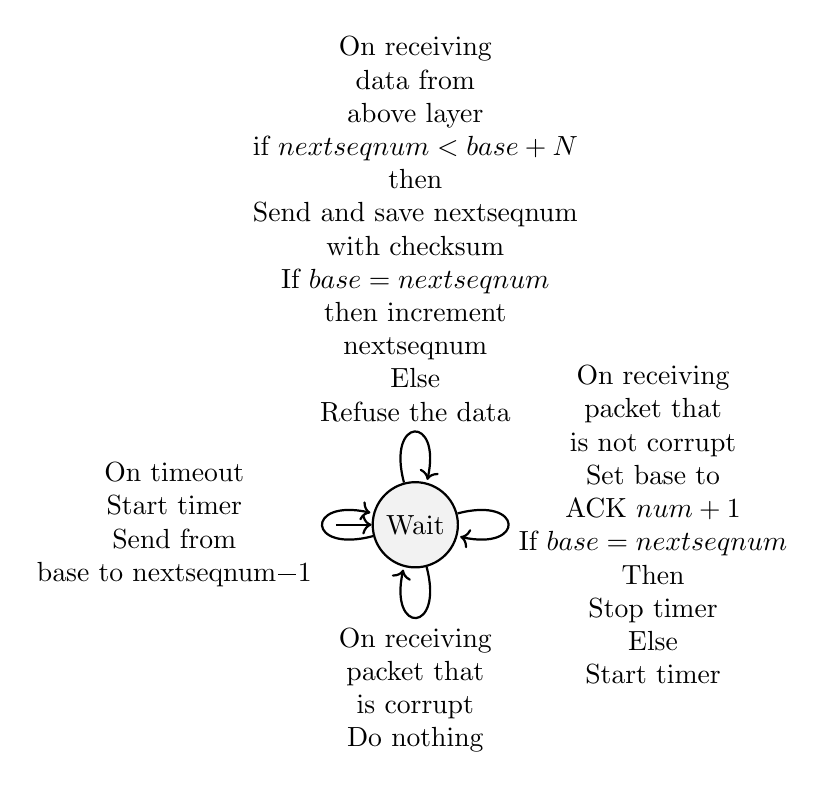
\begin{tikzpicture}[node distance={10cm},thick,main/.style = {draw, circle}]
    \node[state, initial] (wait) {Wait};

    \draw
    (wait) edge[loop above, above]   node[align=center] {On receiving\\data
      from\\above layer\\if $\text{nextseqnum} <
      \text{base}+N$\\then\\Send and save
      \lstinline{nextseqnum}\\with checksum\\ If $\text{base} =
      \text{nextseqnum}$ \\then
      increment\\\lstinline{nextseqnum}\\Else\\Refuse the data
    } (wait)

    (wait) edge[loop left]    node[align=center] {On timeout\\Start
    timer\\Send from\\ \lstinline{base} to \lstinline{nextseqnum-1}} (wait)

    (wait) edge[loop right, right]   node[align=center] {On
      receiving\\packet that\\is not corrupt\\Set \lstinline{base}
      to\\ACK $\text{num} + 1$\\If $\text{base} =
    \text{nextseqnum}$\\Then\\Stop timer\\Else\\Start timer} (wait)

    (wait) edge[loop below]   node[align=center] {On
    receiving\\packet that\\is corrupt\\Do nothing} (wait)

    ;
  \end{tikzpicture}
  \caption{GBN sender, note: $\text{base} = 1$ and $\text{nextseqnum}
  = 1$, initially}
\end{figure}

\begin{figure}[H]
  \centering
  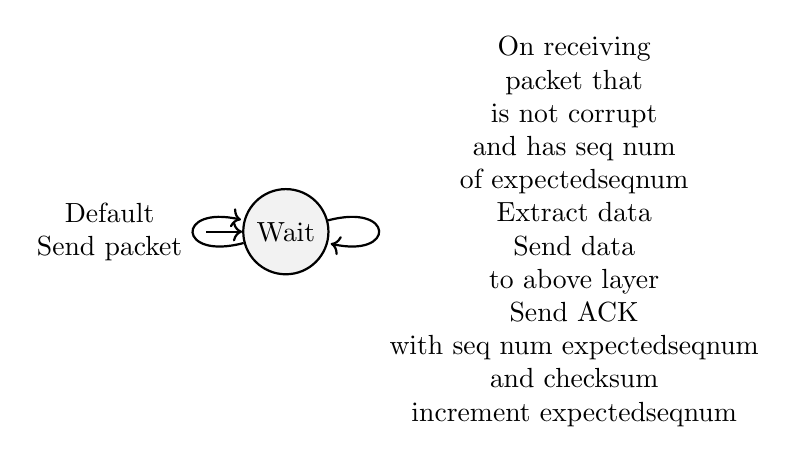
\begin{tikzpicture}[node distance={10cm},thick,main/.style = {draw, circle}]
    \node[state, initial] (wait) {Wait};

    \draw
    (wait) edge[loop right] node[align=center] {On receiving\\packet
      that\\is not corrupt\\and has seq num\\ of
      \lstinline{expectedseqnum}\\Extract data\\Send data\\to above
      layer\\Send ACK\\with seq num \lstinline{expectedseqnum}\\and
    checksum\\increment \lstinline{expectedseqnum}} (wait)

    (wait) edge[loop left] node[align=center] {Default\\Send packet} (wait)

    ;
  \end{tikzpicture}
  \caption{GBN receiver, note: $\text{expectedseqnum} = 0$,
  initially, and first ACK sent will have seq num 0}
\end{figure}

The GBN sender must respond to three types of events:
\begin{description}
  \item[Invocation from above layer] - When data is passed from the
    above layer, the sender first checks to see if the window is
    full, i.e. Whether there are $N$ outstanding, unacknowledged
    packets. If it's not full a packet is created and send and
    variables are appropriately updated. If it is full then the
    sender returns the data back to the above layer, an implicit
    implication that the window is full, and that the above layer
    should try again later.
  \item[Receipt of an ACK] - An acknowledgement for a packet with
    sequence number $n$ will be taken to be a \textbf{cumulative
    acknowledgement}, indicating that all packets with a sequence
    number up to and including $n$ have been correctly received at the receiver.
  \item[Timeout] - As in the stop-and-wait protocol, a timer will be
    used to recover form lost data or acknowledgement packets. If a
    timeout occurs, the send resends all packets that have been
    previously sent but have not yet been acknowledged. If an ACK is
    received but there are still additional transmitted but not yet
    acknowledged packets, the timer is restarted, if there are no
    outstanding, unacknowledged packets the timer is stopped.
\end{description}

The receiver side of GBN is simpler. If a packet with sequence number
$n$ is received correctly and is in order, i.e. the data last
delivered to the upper layer came from a packet with sequence number
$n -1$, the receiver sends an ACK for packet $n$ and delivers the
data portion of the packet to the above layer. In all other cases the
receiver discards the packet and resends an ACK for the most recently
received in-order packet.

The receiver discards out-of-order packets because, since the sender
only sends packets in order, if a packet with sequence number $n$ is
received before a packet with sequence number $n - 1$, the packet
with sequence number $n$ must be a retransmission of a previously
sent packet, and thus the receiver can simply resend an ACK for the
most recently received in-order packet.

There are scenarios where GBN suffers from poor performance, for
example when the window size and bandwidth-delay product are large,
and the sender can have many packets in the pipeline, if a packet is
lost, the sender has to retransmit all packets in the pipeline, even
if only one packet is lost, and the rest of the packets are correctly
received at the receiver, this is known as the \textbf{TCP meltdown problem}.

\subsection{Selected Repeat (SR)}

Selective Repeat protocols avoid unnecessary retransmissions by only
retransmitting those packets that it suspects were received in error
at the receiver. This requires the receiver to individually
acknowledge correctly received packets, and to buffer out-of-order
packets until the missing packets are received and can be delivered
in order to the above layer. A window size if $N$ is again used to
limit the number of in-transit, unacknowledged packets, however
unlike GBN the sender will have already  received ACKs for some of
the packets in the window.

The SR receiver will acknowledge a correctly received packet whether
or not it is in order. Out-of-order packets are buffered until any
missing packets are received at which point a batch of packets can be
delivered in order to the above layer.

The SR sender goes through the following events and actions:
\begin{description}
  \item[Data received from above layer]  - When data is received the
    SR sender checks the next available sequence number for the
    packet. If the sequence number is within the sender's window, the
    data is palletized and sent, otherwise it is either buffered or
    returned to above layer for later transmission.
  \item[Timeout] - Each packet has its own logical timer, since only
    a single packet will be transmitted on timeout.
  \item[ACK received] - If an ACK is received the sender marks that
    packet as received provided it is in the window. If the packet's
    sequence number is equal to \lstinline{send_base}, the window
    base is moved forward to the unacknowledged packet with the
    smallest sequence number. If the window moves and there are
    untransmitted packets with sequence numbers within the window
    those packets are retransmitted.
\end{description}

The SR receiver goes through the following events and actions:
\begin{description}
  \item[Packet with sequence number in rcv\_base, rcv\_base+N-1
    received] - If the packet is correctly
    received, the receiver sends an ACK for that packet and
    buffers the packet if it is out of order. If the packet is in
    order, i.e. its sequence number is equal to \lstinline{rcv_base},
    the receiver delivers the data to the above layer and moves the
    window forward, delivering any buffered packets that are now in
    order.
  \item[Packet with sequence number in rcv\_base, rcv\_base-1 is
    received] - In this case, an ACK is send even though this is a
    packet that the receiver has already acknowledged.
  \item[Otherwise] - Ignore the packet
\end{description}

\chapter{Connection-Oriented Transport: Transmission Control Protocol}

\section{The TCP Connection}

\dfn{Handshaking}{
  Exchanging preliminary segments to establish a connection before
  the actual data transfer begins.
}

TCP is connection oriented because before one process can begin to
send data to another the two must first establish a connection
through \textbf{handshaking}. As part this connection both sides must
initialize many TCP state variables.

\dfn{Full-Duplex Service}{
  If there is a TCP connection between hosts, both hosts can send
  data to each other at the same time, i.e. the connection is
  full-duplex, and the state variables for the two directions of data
  transfer are maintained independently
}

\dfn{Point-to-Point}{
  Connections only exist between a single sender and receiver
}

A TCP connection is a purely logical one, which common state only
residing in the TCPs in the two communicating hosts. TCP provides a
\textbf{full-duplex} service, and is always \textbf{point-to-point}.

A TCP connection is initiated by \textbf{three-way handshake} process
consisting of the following steps:
\begin{description}
  \item[SYN] - A client initiates a connection by sending a TCP
    segment with the SYN
    flag set to 1.
  \item[SYN-ACK] - The server responds to the client's SYN segment by
    sending a TCP segment with both the SYN and ACK flags set to 1.
    The ACK flag is set to acknowledge the client's SYN segment, and
    the SYN flag is set to indicate that the server is also
    initiating a connection.
  \item[ACK] - The client responds to the server's SYN-ACK segment by
    sending a TCP segment with the ACK flag set to 1, acknowledging
    the server's SYN-ACK segment. At this point, the connection is
    established and both sides can begin sending data to each other.
    Usually data is sent with this ACK segment, but it is not required.
\end{description}

Once data is sent from a client through a socket, the data is sent to
the connection's \textbf{send buffer}, from time to time TCP will
take chunks of data from this buffer and pass it to the network
layer, with its size limited by the \textbf{Maximum Segment Size
(MSS)}, which is set by determining the length of the largest link
layer frame that can be sent by the local sending host, i.e. the
\textbf{Maximum Transmission Unit (MTU)}, and setting the MSS to
ensure that an encapsulated TCP segment plus the TCP/IP header length
will fit into a single link layer frame.

TCP pairs each chunk of client data with a TCP header, forming a TCP
segment, which is then passed to the network layer for transmission.

\section{TCP Segment Structure}

A TCP segment consists of the following fields:
\begin{description}
  \item[Source Port] - 16 bits used to identify the sending process
  \item[Destination Port] - 16 bits used to identify the receiving process
  \item[Checksum] - 16 bits used for error detection
  \item[Sequence Number] - 32 bits used for implementing reliable data transfer
  \item[Acknowledgement Number] - 32 bits used for implementing
    reliable data transfer
  \item[Receive Window] - 16 bits used for flow control
  \item[Header Length] - 4 bits used to indicate the length of the TCP header
  \item[Options Field] - Optional field used for various purposes,
    such as indicating the MSS
    or as a window scaling factor for high speed networks,
  \item[Flags] - 6 bits used for indicating various control flags such as:
    \begin{description}
      \item[ACK]  - Indicates the value carried in the
        acknowledgement number field is valid
      \item[RST] - Used in connection setup and teardown
      \item[SYN] - Used in connection setup
      \item[FIN] - Used in connection teardown
      \item[PSH] - Indicates that the receiver should pass the data
        to the upper layer immediately
      \item[URG] - Indicates that the urgent pointer field is valid
    \end{description}
\end{description}

\subsection{Sequence Number and Acknowledgement Numbers}

The sequence and acknowledgement numbers are used to implement
reliable data transfer in TCP. TCP views data as an unstructured but
ordered stream of bytes, sequence numbers follows this view in that
they are counted over the stream of bytes not over the stream of
segments, i.e. the sequence number for a segment is the byte steam
number of the first byte in the segment's data section.

\dfn{Cumulative Acknowledgement}{
  An acknowledgement that acknowledges not only the segment it is
  acknowledging but also all segments with a sequence number less than
  the acknowledged segment.
}

The acknowledgement number that a host puts in its ACK segment is the
sequence number of the next byte that it expects to receive from the
other host, i.e. the byte stream number of the first byte that has
not yet been received. This follows that if a host receives a segment
with a sequence number of $n$ and data length of $l$ the
acknowledgement number that it will send back in its ACK segment is
\[
  \text{ACK number} = n + l
\]
This TCP provides \textbf{cumulative acknowledgements}

\section{Round Trip Time (RTT) Estimation and Timeout}

TCP uses timeout/retransmission mechanisms to recover from lost
segments, and thus it is important to set the timeout interval
appropriately, if the timeout interval is too short, TCP will
unnecessarily retransmit segments that are not lost, and if it is too
long, TCP will be slow to recover from lost segments.

\subsection{Estimating the RTT}

TCP estimates the RTT as follows:

Given the sample RTT, denoted as \lstinline{SampleRTT}, for a segment
is the amount of time between when the segment is sent, and when an
acknowledgement for the segment is received, most  TCP
implementations take one \lstinline{SampleRTT} measurement at a time,
and use an exponentially weighted moving average to compute the
estimated RTT, denoted as \lstinline{EstimatedRTT}, as follows:
\begin{align*}
  \text{\lstinline{EstimatedRTT}} = (1 - \alpha) \times
  \text{\lstinline{EstimatedRTT}} + \alpha \times \text{\lstinline{SampleRTT}}
\end{align*}
This is an iterative process, with the initial value of
\lstinline{EstimatedRTT} set to the first \lstinline{SampleRTT}
measurement, and $\alpha = 0.125$ typically.

In addition the \textbf{deviation} of the RTT, denoted as
\lstinline{DevRTT}, is also estimated like so:
\begin{align*}
  \text{\lstinline{DevRTT}} = (1 - \beta) \times
  \text{\lstinline{DevRTT}} + \beta \times  \mid \text{\lstinline{SampleRTT}} -
  \text{\lstinline{EstimatedRTT}} \mid
\end{align*}
With $\beta = 0.25$ typically.

\subsection{Setting and Managing the Retransmission Timeout Interval}

Given the values of \lstinline{EstimatedRTT} and \lstinline{DevRTT},
the \lstinline{TimeoutInterval} is set as follows:
\begin{align*}
  \text{\lstinline{TimeoutInterval}} =
  \text{\lstinline{EstimatedRTT}} + 4 \times
  \text{\lstinline{DevRTT}}
\end{align*}

An initial \lstinline{TimeoutInterval} is set to 1 second, and the
timeout interval is only updated for segments that are not
retransmitted, since retransmitted segments may have an artificially
large \lstinline{SampleRTT} due to the time spent waiting for the
timeout to occur.

This formula sets the timeout interval to be large enough to account
for variations in the RTT, thus avoiding unnecessary retransmissions,
while still being responsive enough to recover from lost segments in
a timely manner.

\section{Reliable Data Transfer}

TCP creates a reliable data transfer service on top of the unreliable
IP layer, and thus it must have mechanisms to detect and recover from
lost segments, corrupted segments and excessively delayed segments.

TCP uses the reliable data transfer mechanisms of checksums, sequence
numbers, acknowledgements, retransmissions and timers to achieve
this, but overcomes the theoretical overhead of multiple timers used
in the most robust reliable data transfer protocols by using a single
retransmission timer.

A TCP sender generally reacts and responds to three types of events,
disregarding flow or congestion control.
\begin{description}
  \item[Data received fom above layer] - When data is received from
    above a TCP segment is created with the sequence number
    \lstinline{NextSeqNum}, and a checksum, if the retransmit timer
    is not running it is started and the segment is sent, with
    \lstinline{NextSeqNum} increasing by the length of the data in the segment.
  \item[Timeout] - Once a timeout occurs, the unacknowledged segment
    with the smallest sequence number is retransmitted, and the timer
    is restarted.
  \item[ACK received with ACK field value of $y$] - If $y$ is greater
    than \lstinline{SendBase}
    \lstinline{SendBase} is set to $y$, and if there are still
    unacknowledged segments the timer is started.
\end{description}

The timeout time is \lstinline{TimeoutInterval}, and the timer is
only started when the first unacknowledged segment is sent, and is
stopped when all segments are acknowledged, thus only one timer is needed.

\subsection{Doubling the Timeout Interval}

Most TCP implementations use an exponential back off strategy to
provide a limited form of congestion control, in which once a timeout
occurs the next timeout interval is set to be twice the previous
timeout interval. However whenever the timer is started after a
timeout, i.e. it receives data from the above layer, or it receives
an ACK for a segment, the timeout interval is reset to the value
computed from the RTT estimation process.

This works on the logic that the timer expiration is most likely
caused by congestion in the network, and thus doubling the timeout
interval will help to reduce the likelihood of another timeout
occurring, and thus help to reduce congestion in the network.

\subsection{Fast Retransmit}

\dfn{Duplicate ACK}{
  An ACK that reacknowledges a segment that has already been
  acknowledged, i.e. an ACK with an ACK number that is less than the
  ACK number of the most recently acknowledged segment.
}

A problem with timeout trigged retransmission is that the timeout
period could be long. To solve this the sender can be made to detect
packet loss before the timeout event, by recording duplicate ACKs,
and if three duplicate ACKs are received, i.e. four ACKs with the
same ACK number, the sender can infer that a segment has been lost and
retransmit the segment that is suspected to be lost, this is known as
\textbf{fast retransmit}.

\begin{table}[H]
  \begin{center}
    \begin{tabularx}{\textwidth}{|X|X|}
      \hline
      Event & TCP Receiver Action \\
      \hline
      Arrival of in order segment with expected sequence number. All
      data up to expected sequence number already acknowledged  &
      Delayed ACK. Wait up to 500 ms for arrival of another in order
      segment. If next in order segment does not arrive within this
      interval send an ACK  \\
      \hline
      Arrival of in order segment with expected sequence number. One
      other in order segment waiting for ACK transmission &
      immediately send single cumulative ACK, ACKing both in order segments \\
      \hline
      Arrival of out of order segment with higher than expected
      sequence number. Gap detected & immediately send duplicate ACK,
      indicating sequence number of next expected byte, i.e. lower
      end of the gap \\
      \hline
      Arrival of segment that partially or completely fills in gap in
      received data & immediately send ACK, provided that segment
      starts at the lower end of the gap. \\
      \hline
    \end{tabularx}
  \end{center}
  \caption{TCP ACK Generation}\label{tab:}
\end{table}

\subsection{GBN or SN}

TCP has features of both GBN and SN, and is best categorized as a
hybrid of the two, due to the following features:
\begin{description}
  \item[GBN]-
    \begin{itemize}
      \item TCP uses cumulative acknowledgements
      \item Correctly received but out of order segments are not
        individually ACKed by the receiver
      \item The TCP sender bys only maintain the smallest sequence
        number of a transmitted but unacknowledged byte
        (\lstinline{SendBase}) and the sequence number of the next
        byte to be sent (\lstinline{NextSeqNum})
    \end{itemize}
  \item[SN] -
    \begin{itemize}
      \item TCP uses a single retransmission timer, and thus only retransmits
        one segment at a time, even if multiple segments are suspected
        to be lost.
      \item Many TCP implementations buffer correctly received but
        out of order segments.
      \item TCP can selectively retransmit segments that are
        suspected to be lost based on the
        number of duplicate ACKs received, and thus does not have to
        wait for a timeout event to occur before retransmitting a
        segment that is suspected to be lost.
    \end{itemize}
\end{description}

\section{Flow Control}

TCP provides flow control to ensure that a sender does not risk
overflowing the receivers buffer. Flow control is a speed matching
service, matching the rate at which the sender is sending against the
rate at which the receiver is reading.

Flow control differs from congestion control in that flow control is
end-to-end, between hosts, and used to prevent the sender from
overwhelming the receiver, while congestion control aims to prevent
the sender from overwhelming the network, and is thus a host-to-network service.

TCP provides flow control by having the sender maintain a
\textbf{receive window} state variable, which is used to give the
sender an upper bound of how much free buffers space is available at
the receiver, and thus how much data the sender can have in transit
without overwhelming the receiver. Because TCP is full-duplex the
sender et each side of the connection maintains its own receive window.

Below is how the receive window operates, given a sending host A, and
a receding host B, sending data over a TCP connection from A to B:
\begin{itemize}
  \item Host B allocates a receive buffer to this connection, with
    its size denoted as \lstinline{RcvBuffer}, intermittently reading
    from this buffer.
  \item \lstinline{LastByteRead} is the number of last byte in the
    data stream read from the buffer by the application process in B.
  \item \lstinline{LastByteRcvd} is the number of the last byte in
    the data stream that has arrived from the network and has been
    placed in the receive buffer at B.
  \item TCP cannot overflow the receive buffer, therefore
    \begin{align*}
      \mbox{\lstinline{LastByteRcvd}} - \mbox{\lstinline{LastByteRead}} \leq
      \mbox{\lstinline{RcvBuffer}}
    \end{align*}
  \item Thus the receive window, denoted by \lstinline{rwnd}, set to
    the amount of space left in the buffer
    \begin{align*}
      \text{\lstinline{rwnd}} = \mbox{\lstinline{RcvBuffer}} -
      (\mbox{\lstinline{LastByteRcvd}} - \mbox{\lstinline{LastByteRead}})
    \end{align*}
  \item Host A keeps track of the last byte sent, denoted as
    \lstinline{LastByteSent}, and the last byte acknowledged, denoted
    as \lstinline{LastByteAcked}, and by keeping the amount of
    unacknowledged data less than the value of \lstinline{rwnd} it
    can ensure that it does not overflow the buffer at B, i.e. ensuring that
    \begin{align*}
      \text{\lstinline{LastByteSent}} -
      \text{\lstinline{LastByteAcked}} \leq \text{\lstinline{rwnd}}
    \end{align*}
\end{itemize}

The value of \lstinline{rwnd} is sent by B to A in the header of ACK
segments allowing A to adapt its sending rate to the rate at which B
is reading from the buffer.

This approach however can suffer from the \textbf{zero window
problem}, where the host B's receive buffer becomes full so that
$\text{\lstinline{rwnd}} = 0$, and thus host A cannot send any more data
until B reads from the buffer and sends an ACK with a non-zero
\lstinline{rwnd} value, but if the ACK with the non-zero
\lstinline{rwnd} value is lost, then host A will be stuck waiting for
an ACK that will never arrive, thus causing a deadlock. To solve
this, host A can periodically send a probe segment to host B to check
if the receive window has opened up, and thus avoid the zero window problem.

\section{Connection Management}

TCP connections are merely an abstraction and thus must be explicitly
created and destroyed by the communicating hosts. TCP goes through
the following process to establish a connection:
\begin{enumerate}
  \item  The client sends a SYN segment, containing no application
    data, with the SYN flag bit set to 1, and a randomly chosen
    initial sequence number \lstinline{client_isn} to the server.
  \item The server receives the SYN segment, allocates the TCP
    buffers and variables and sends a connection-granted segment to
    the TCP client, with the SYN and ACK flag bits set to 1, with an
    acknowledgement number of $\text{\lstinline{client_isn}} + 1$, and a
    randomly chosen initial sequence number \lstinline{server_isn}.
    This is a SYN-ACK segment.
  \item The client receives the SYN-ACK segment, allocates the TCP buffers
    and variables, and sends an ACK segment to the server, with the ACK
    flag bit set to 1, and an acknowledgement number of
    $\text{\lstinline{server_isn}} + 1$. This is an ACK segment, and once
    the server receives this segment the connection is established
    and both sides can begin sending data to each other, although in
    practice data is usual sent with the ACK segment in step 3.
\end{enumerate}

When a TCP connection is no longer needed, it must be explicitly closed by
the communicating hosts, and TCP goes through the following process to
close a connection:
\begin{enumerate}
  \item Either the client or the server can initiate the connection
    termination process
    by sending a FIN segment, with the FIN flag bit set to 1, and an
    appropriate sequence number.
  \item The other host receives the FIN segment, and sends an ACK
    segment to acknowledge the FIN segment, with the ACK flag bit set
    to 1, and an
    acknowledgement number of the sequence number of the FIN segment
    plus 1.
  \item The host that sent the ACK segment in step 2, sends a FIN segment to
    the other host, with the FIN flag bit set to 1, and an appropriate
    sequence number.
  \item  The host that sent the FIN segment in step 3, receives the FIN
    segment, and sends an ACK segment to acknowledge the FIN segment, with
    the ACK flag bit set to 1, and an acknowledgement number of the
    sequence number of the FIN segment plus 1. Once this ACK segment is
    received by the host that sent the FIN segment in step 3, the connection is
    fully closed and all resources allocated to the connection can be
    released.
\end{enumerate}

During a connection's lifetime a TCP client can be in one of the
following states:
\begin{description}
  \item[CLOSED]  - No connection exists, the initial state of a TCP connection
  \item[SYN\_SENT] - A SYN segment has been sent, but the connection is not yet
    established. The client waits for a SYN-ACK segment from the
    server. On receiving it it sends an ACK segment and moves to the
    ESTABLISHED state.
  \item[ESTABLISHED] - The connection is established and both sides
    can send data
  \item[FIN\_WAIT\_1] - A FIN segment has been sent, but the
    connection is not yet
    fully closed. The client waits for an ACK segment from the server. On
    receiving it, the client moves to the FIN\_WAIT\_2 state.
  \item[FIN\_WAIT\_2] - The client waits for a FIN segment from the server. On
    receiving it, the client sends an ACK segment and moves to the
    TIME\_WAIT state.
  \item[TIME\_WAIT] - The client waits for a period of time, typically
    2 times the maximum segment lifetime, to ensure that any delayed
    segments in the network have time to arrive and be discarded
    before the connection is fully closed and all resources allocated
    to the connection can be released.
\end{description}

The server can be in one of the following states:
\begin{description}
  \item[CLOSED]  - No connection exists, the initial state of a TCP
    connection, server creates a listen socket.
  \item[LISTEN] - The server is waiting for a connection request from
    any client. On receiving a SYN segment from a client, the server
    sends a SYN-ACK segment to the client and moves to the SYN\_RCVD state.
  \item[SYN\_RCVD] - The server has received a SYN segment from a client, and
    has sent a SYN-ACK segment to the client, but the connection is not yet
    established. The server waits for an ACK segment from the client. On
    receiving it, the server moves to the ESTABLISHED state.
  \item[ESTABLISHED] - The connection is established and both sides
    can send data
  \item[CLOSE\_WAIT] - The server has received a FIN segment from the
    client, and has sent an ACK segment to the client, but the
    connection is not yet fully closed. The server waits for a FIN
    segment from the client. On receiving it, the server sends an ACK
    segment to the client and moves to the LAST\_ACK state.
  \item[LAST\_ACK] - The server has sent a FIN segment to the
    client, and is waiting for an ACK segment from the client. On
    receiving it, the server moves to the CLOSED state and all resources
    allocated to the connection can be released.
\end{description}

\section{Congestion Control}

\subsection{Causes and Costs of Congestion}

\subsubsection{Two Senders, a Router with Infinite Buffers}

\subsubsection{Two Senders and a Router with Finite Buffers}

\subsubsection{Four Senders, Routers with Finite Buffers and Multi-hop Paths}

\subsection{Approaches to Congestion Control}

\chapter{TCP Congestion Control}

\section{Classic TCP Congestion Control}

\subsection{Slow Start}

\subsection{Congestion Avoidance}

\subsection{Fast Recovery}

\subsection{Retrospective}

\subsection{TCP Cubic}

\subsection{TCP Reno}

\section{Network-Assisted Explicit Congestion Notification and
Delayed-based Congestion Control}

\subsection{Explicit Congestion Notification}

\subsection{Delay-based Congestion Control}

\section{Fairness}

\subsection{Fairness and UDP}

\subsection{Fairness and Parallel TCP Connections}

\end{document}
